\documentclass[tikz, border=4pt]{standalone}
\usepackage[T1]{fontenc}
\usepackage{lmodern}
\usetikzlibrary{arrows.meta, positioning, fit, backgrounds}

\definecolor{accent}{HTML}{2F5D8C}
\definecolor{groupfill}{HTML}{EEF3F8}
\definecolor{taskfill}{HTML}{FFFFFF}
\definecolor{note}{HTML}{555555}

\newcommand{\sub}{\tiny\color{note}}
\begin{document}
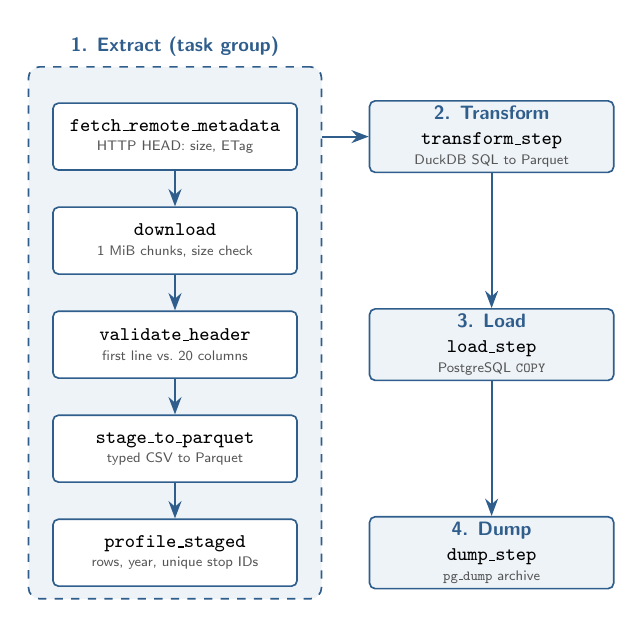
\begin{tikzpicture}[
    font=\sffamily\scriptsize,
    task/.style={draw=accent, fill=taskfill, rounded corners=2pt, line width=0.6pt,
                 minimum width=31mm, minimum height=8.5mm, align=center, inner sep=2pt},
    stage/.style={task, fill=groupfill},
    flow/.style={-{Stealth[length=2.2mm]}, accent, line width=0.7pt},
    group/.style={draw=accent, dashed, rounded corners=4pt, line width=0.6pt, fill=groupfill, inner sep=3mm},
    lbl/.style={font=\sffamily\scriptsize\bfseries, text=accent},
    node distance=4.5mm,
]

\node[task] (meta) {\texttt{fetch\_remote\_metadata}\\[-1pt]{\sub HTTP HEAD: size, ETag}};
\node[task, below=of meta] (dl) {\texttt{download}\\[-1pt]{\sub 1 MiB chunks, size check}};
\node[task, below=of dl] (hdr) {\texttt{validate\_header}\\[-1pt]{\sub first line vs.\ 20 columns}};
\node[task, below=of hdr] (stage) {\texttt{stage\_to\_parquet}\\[-1pt]{\sub typed CSV to Parquet}};
\node[task, below=of stage] (prof) {\texttt{profile\_staged}\\[-1pt]{\sub rows, year, unique stop IDs}};

\draw[flow] (meta) -- (dl);
\draw[flow] (dl) -- (hdr);
\draw[flow] (hdr) -- (stage);
\draw[flow] (stage) -- (prof);

\begin{scope}[on background layer]
  \node[group, fit=(meta)(prof), inner ysep=3mm, yshift=1.5mm] (ext) {};
\end{scope}
\node[lbl, anchor=south] at (ext.north) {1. Extract (task group)};

\node[stage, right=9mm of meta] (tr) {{\bfseries\color{accent}2. Transform}\\[1pt]\texttt{transform\_step}\\[-1pt]{\sub DuckDB SQL to Parquet}};
\node[stage, right=9mm of hdr] (ld) {{\bfseries\color{accent}3. Load}\\[1pt]\texttt{load\_step}\\[-1pt]{\sub PostgreSQL \texttt{COPY}}};
\node[stage, right=9mm of prof] (dp) {{\bfseries\color{accent}4. Dump}\\[1pt]\texttt{dump\_step}\\[-1pt]{\sub \texttt{pg\_dump} archive}};

\draw[flow] (ext.east |- tr.west) -- (tr.west);
\draw[flow] (tr) -- (ld);
\draw[flow] (ld) -- (dp);

\end{tikzpicture}
\end{document}
